\section{显微镜物镜的系统化设计}

\subsection{机械约束与基本构型}

\englishtitle{Mechanical Constraints Behind Microscope Objectives}
\begin{frame}{物镜不是纯光学问题，而是“光学+机械”共同约束}
    \small
    \begin{columns}[T]
        \begin{column}{.50\textwidth}
            \begin{figure}
                \centering
                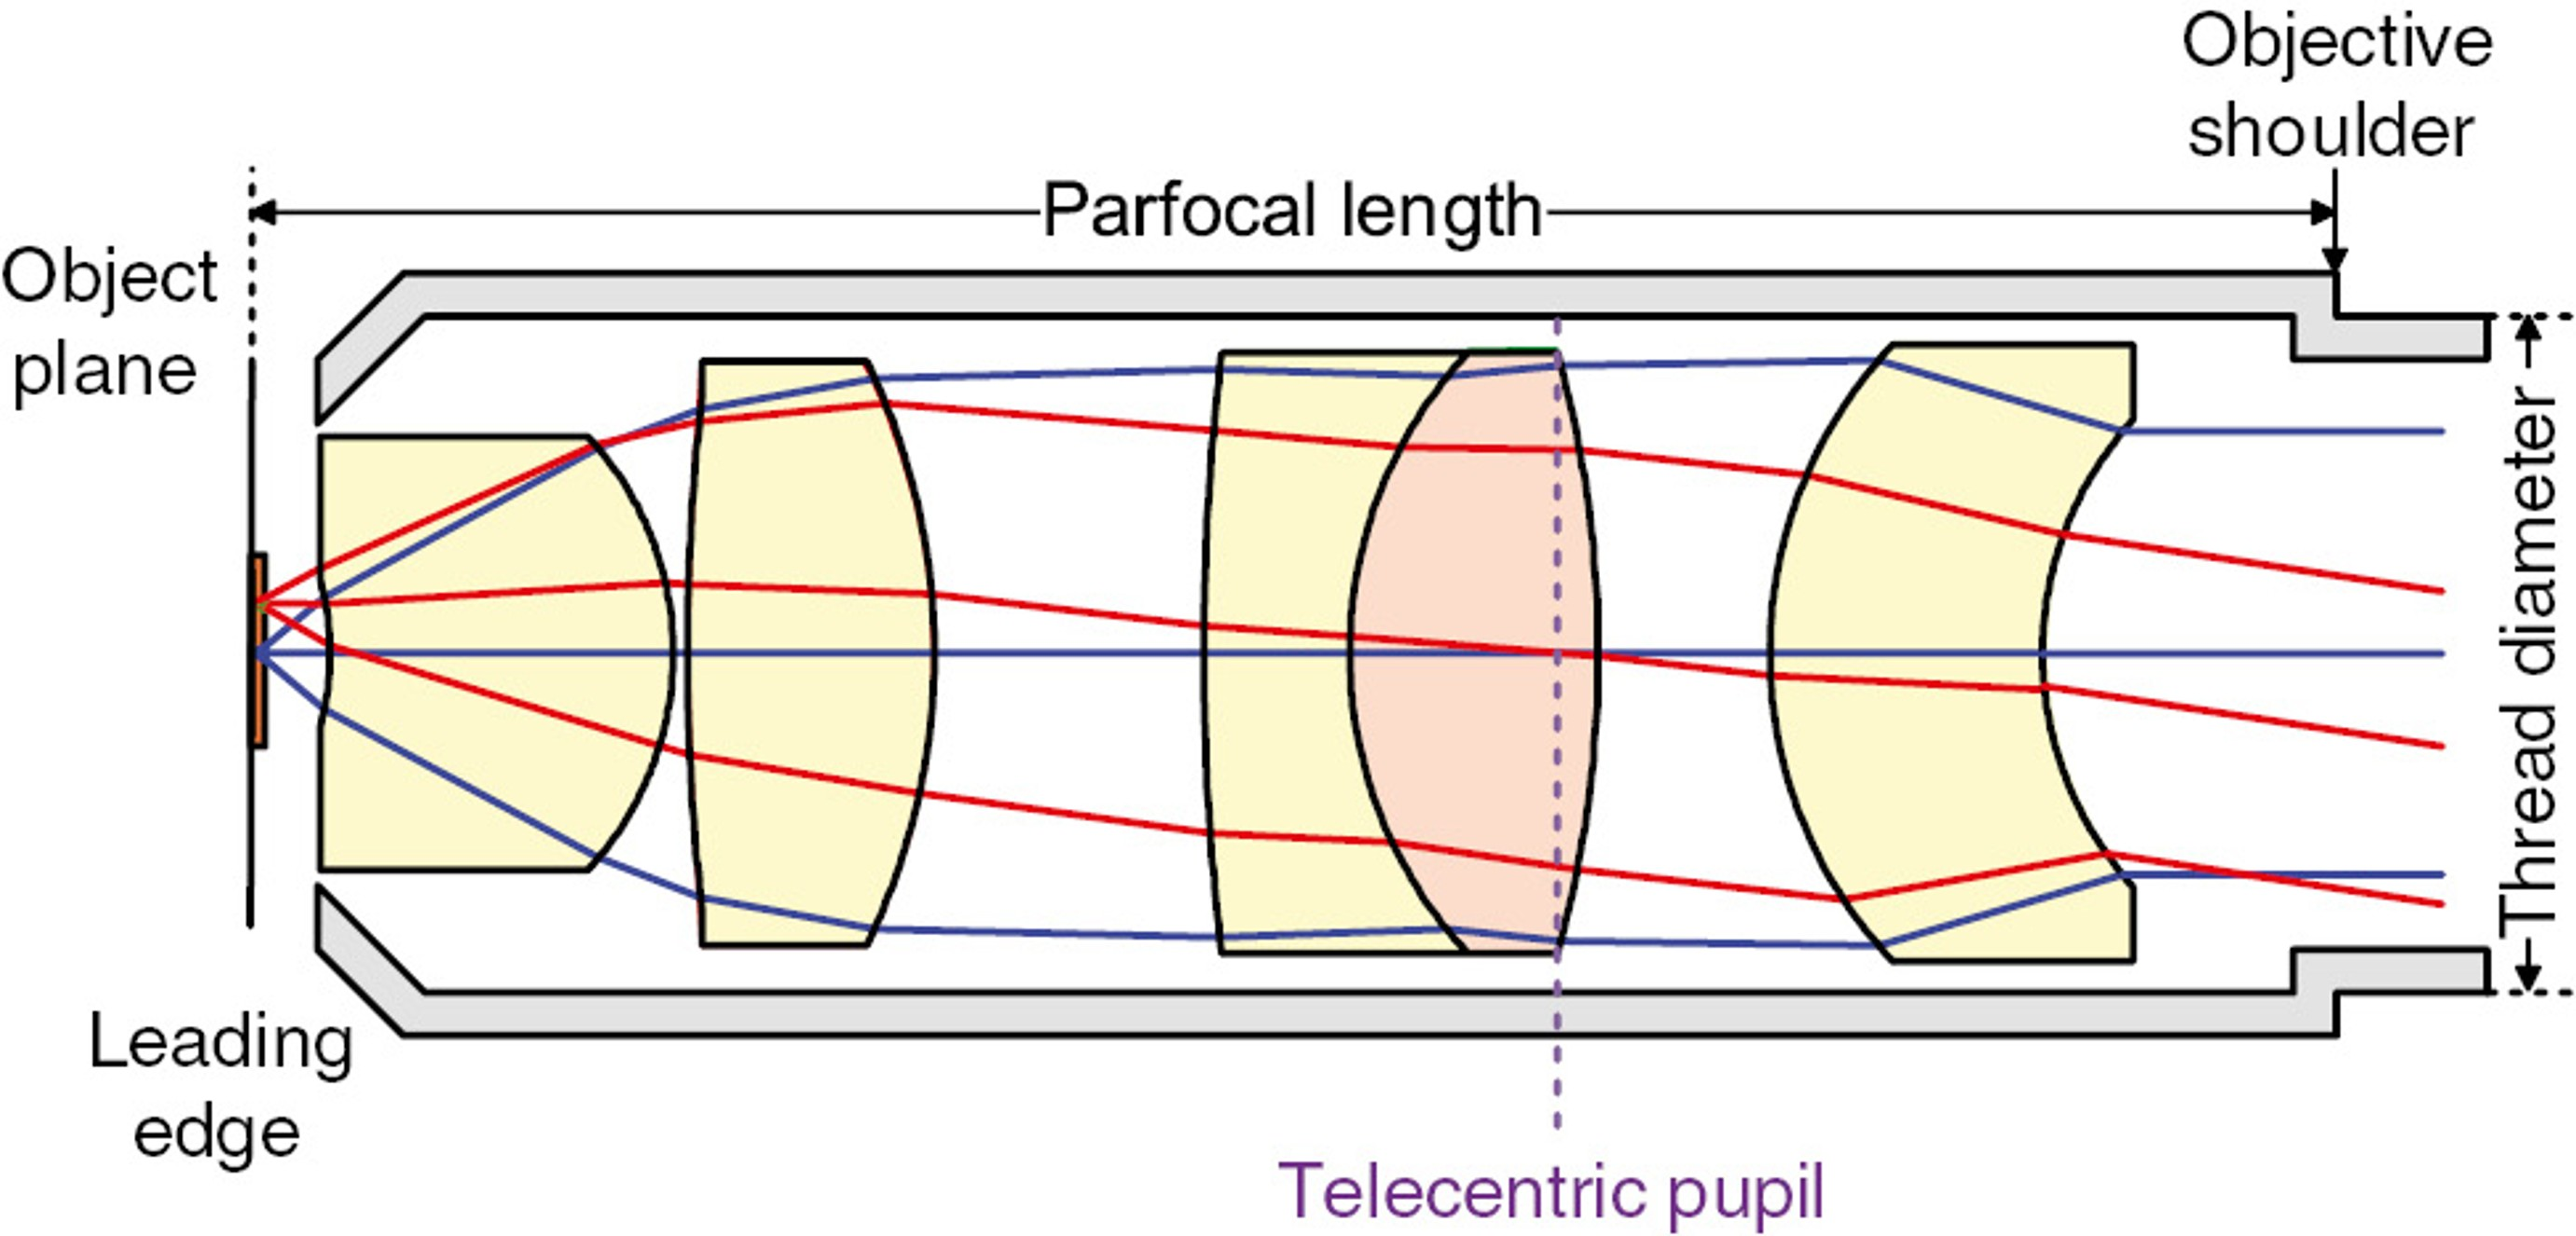
\includegraphics[width=\textwidth,height=0.54\textheight,keepaspectratio]{Figure/Zhang/ZhangFig_01.png}
                \label{fig:zhang_mechanics}
            \end{figure}
        \end{column}
        \hfill
        \begin{column}{.48\textwidth}
            \textbf{图中给出的三个关键机械约束：}
            \begin{itemize}
                \item \alert{Parfocal length（齐焦距）}：样品面到物镜肩部的距离，限制轴向可用空间
                \item \alert{Thread diameter（螺纹直径）}：限制后端光束与出瞳尺寸
                \item \alert{Telecentric pupil（后焦面附近光阑）}：保证物方远心，便于倍率和照明标准化
            \end{itemize}

            \bigbreak
            \textbf{这意味着：}
            \begin{itemize}
                \item 物镜设计从一开始就不是“自由堆镜片”
                \item 高 NA 和大视场会同时挤压\alert{长度}与\alert{口径}预算
                \item 高复杂度物镜常需要更长齐焦距和更大接口
            \end{itemize}

            \alert{设计启示：}显微物镜的结构演化，很多时候不是像差理论先推动，而是\textbf{标准化机械边界逼出来的折中结果}。
        \end{column}
    \end{columns}
\end{frame}

\subsection{19世纪：基础结构的建立}

\englishtitle{From Lister to Abbe: The Origin of Modern Objectives}
\begin{frame}{从 Lister 到 Abbe：现代显微物镜的起点}
    \small
    \begin{columns}[T]
        \begin{column}{.54\textwidth}
            \begin{figure}
                \centering
                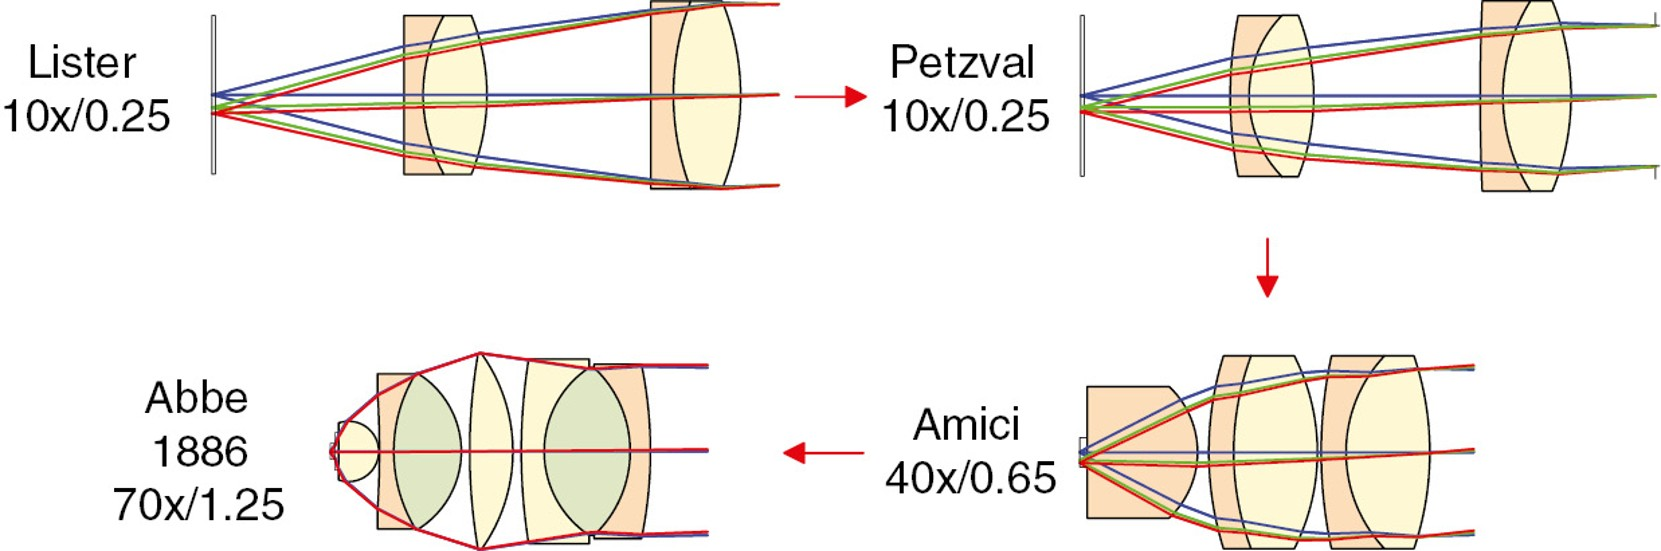
\includegraphics[width=\textwidth,height=0.56\textheight,keepaspectratio]{Figure/Zhang/ZhangFig_02.png}
                \label{fig:zhang_19century}
            \end{figure}
        \end{column}
        \hfill
        \begin{column}{.44\textwidth}
            \textbf{论文中的演化主线非常清楚：}
            \begin{itemize}
                \item \textbf{Lister 1830}：引入消色差双胶合透镜，可视为现代物镜起点
                \item \textbf{Petzval 1843}：优化双组间隔与面形，进一步压低球差、彗差和像散
                \item \textbf{Amici 1850}：加入前端 aplanatic 透镜，把 NA 推向更高水平
                \item \textbf{Abbe 1886}：借助 Schott 玻璃与异常色散材料，做出早期油浸 apochromat
            \end{itemize}

            \bigbreak
            \textbf{核心趋势：}
            \begin{itemize}
                \item 先解决\alert{轴上色差与球差}
                \item 再逐步追求\alert{更高 NA}
                \item 更高 NA 又会反过来恶化\alert{场曲与视场}
            \end{itemize}

            \alert{一句话概括：}显微物镜最早的历史，本质上就是\textbf{“高 NA 能力”和“可用视场”之间的拉扯}。
        \end{column}
    \end{columns}
\end{frame}

\subsection{20世纪：现代结构分化}

\englishtitle{Modern Evolution: Field Flattening, Long WD and PNP}
\begin{frame}{20 世纪的现代结构演化：平场化、长工作距与超低倍}
    \small
    \begin{columns}[T]
        \begin{column}{.58\textwidth}
            \begin{figure}
                \centering
                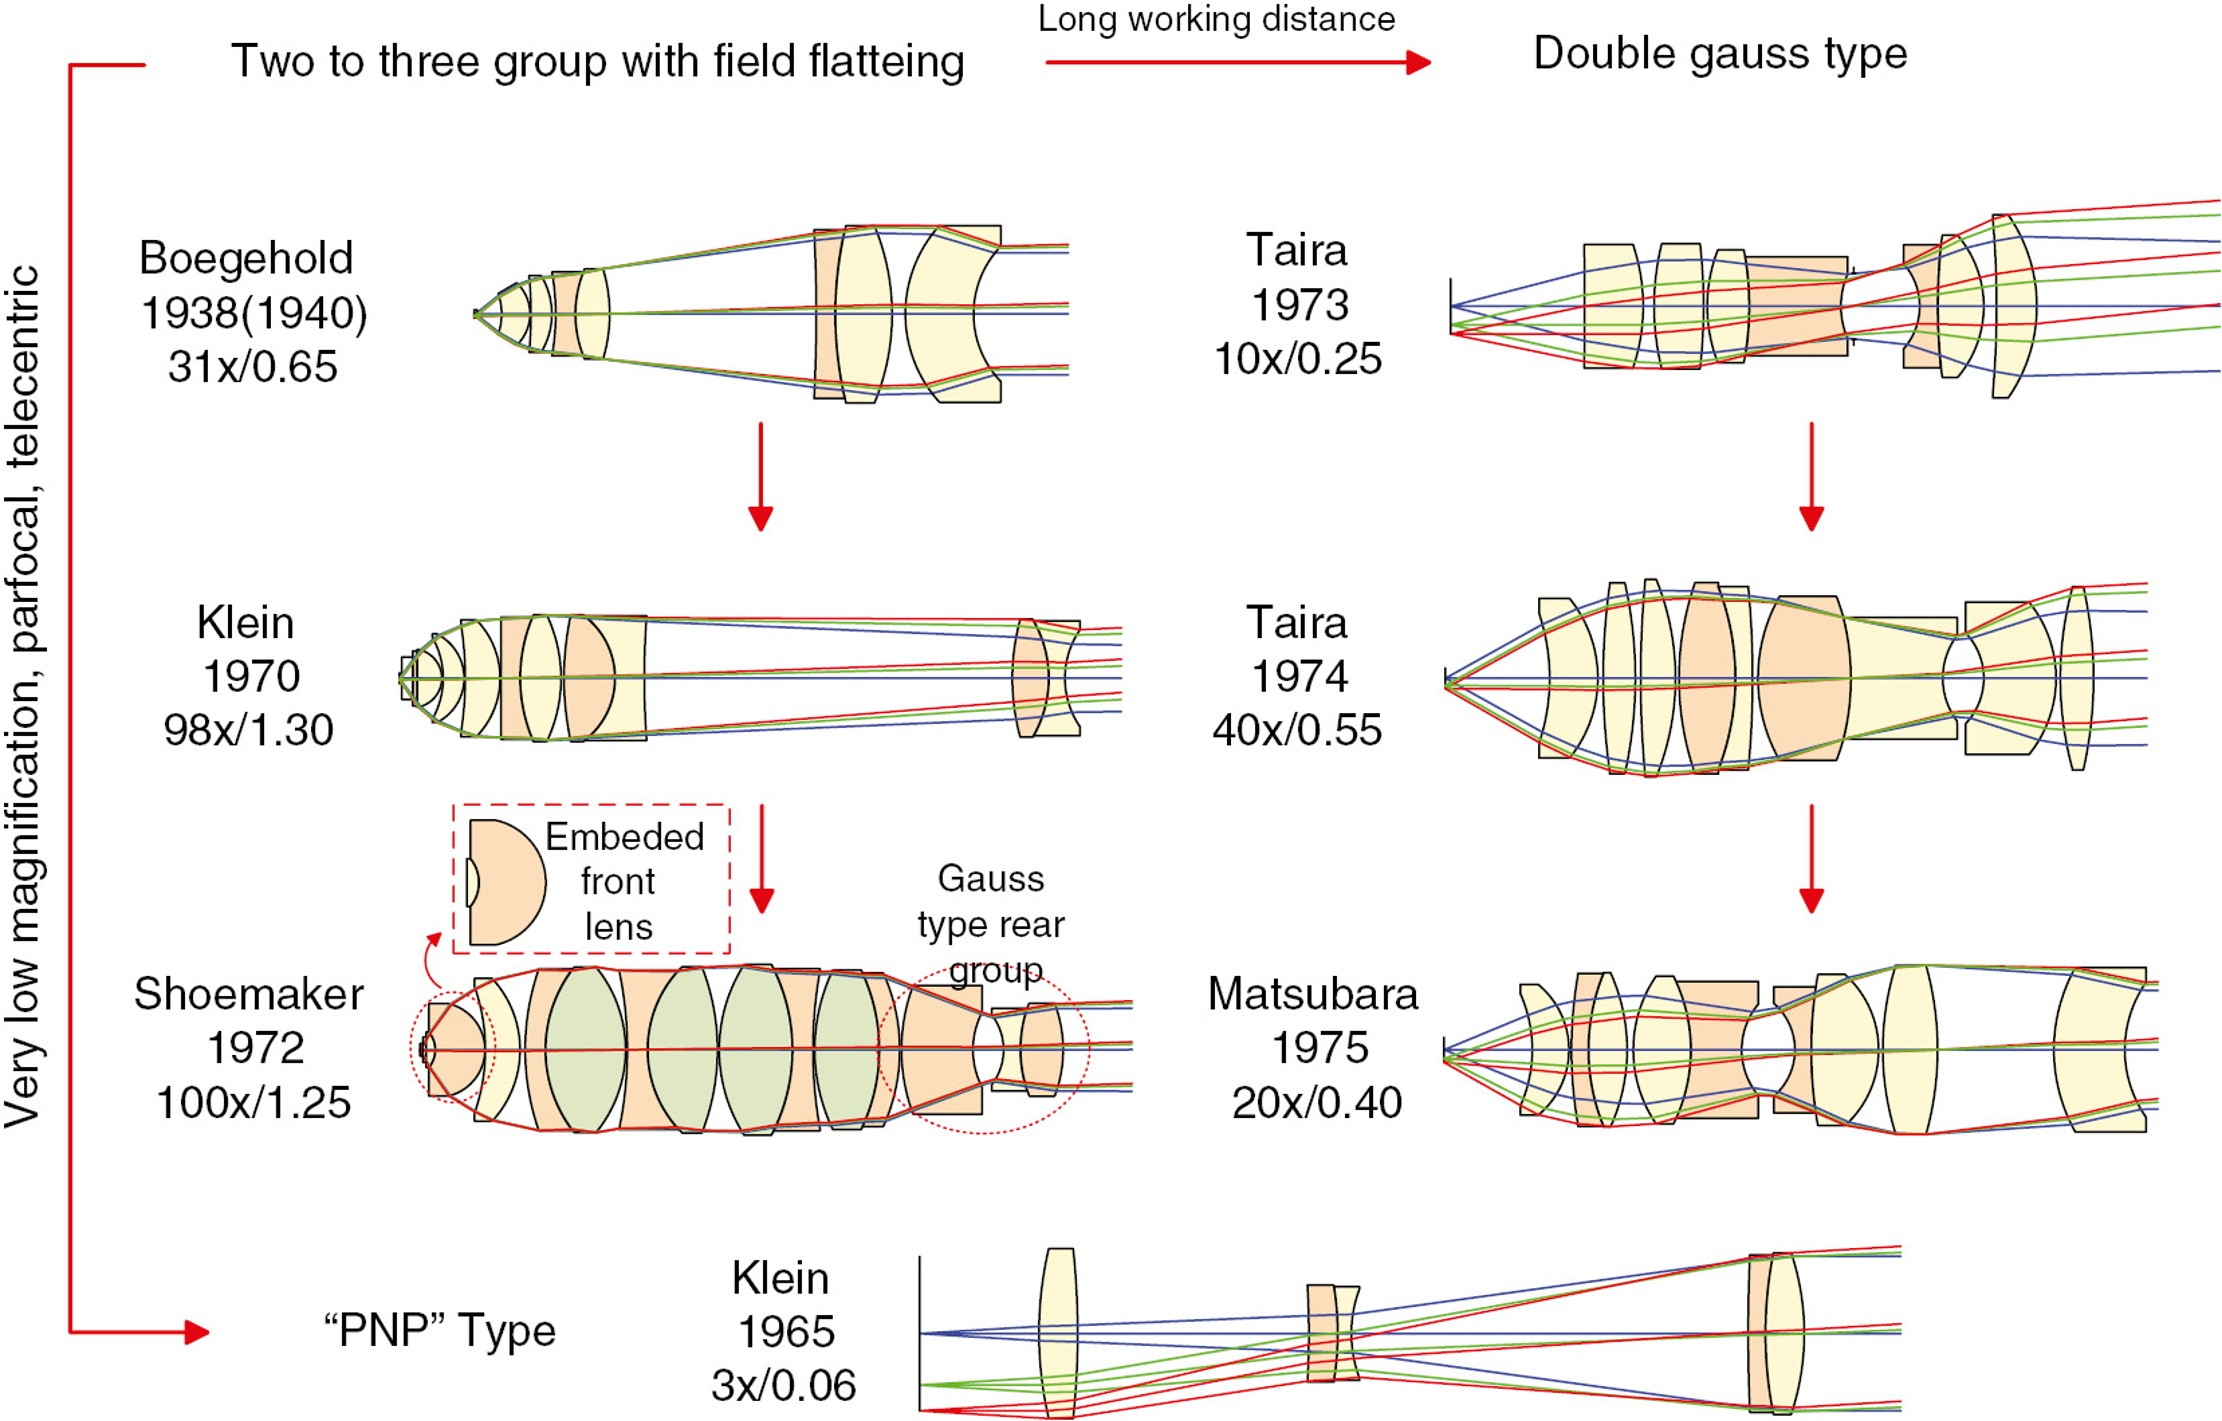
\includegraphics[width=\textwidth,height=0.58\textheight,keepaspectratio]{Figure/Zhang/ZhangFig_03.png}
                \label{fig:zhang_modern_evolution}
            \end{figure}
        \end{column}
        \hfill
        \begin{column}{.40\textwidth}
            \textbf{图里其实包含了三条结构路线：}
            \begin{itemize}
                \item \textbf{平场化路线}：后组厚弯月透镜用于补偿 Petzval 场曲
                \item \textbf{长工作距路线}：把摄影镜头里的 \alert{Double-Gauss} 思想引入物镜
                \item \textbf{超低倍路线}：\alert{PNP} 结构同时满足远心与齐焦
            \end{itemize}

            \bigbreak
            \textbf{这页最值得记住的结论：}
            \begin{itemize}
                \item 高 NA 物镜逐渐从“双组”走向更清晰的\alert{前组-中组-后组}分工
                \item 低倍、大工作距、平场需求并不会自动兼容，往往需要\alert{专门结构}
                \item 这一时期已经出现今天仍在沿用的“清晰三组”范式
            \end{itemize}

            \alert{设计启示：}应用目标不同，主导结构也不同，\textbf{不存在一套万能物镜架构}。
        \end{column}
    \end{columns}
\end{frame}

\subsection{色差校正等级与复杂度代价}

\englishtitle{Chromatic Correction Classes and Their Structural Cost}
\begin{frame}{从 Achromate 到 Superapochromate：校正等级越高，结构越复杂}
    \small
    \begin{columns}[T]
        \begin{column}{.56\textwidth}
            \begin{figure}
                \centering
                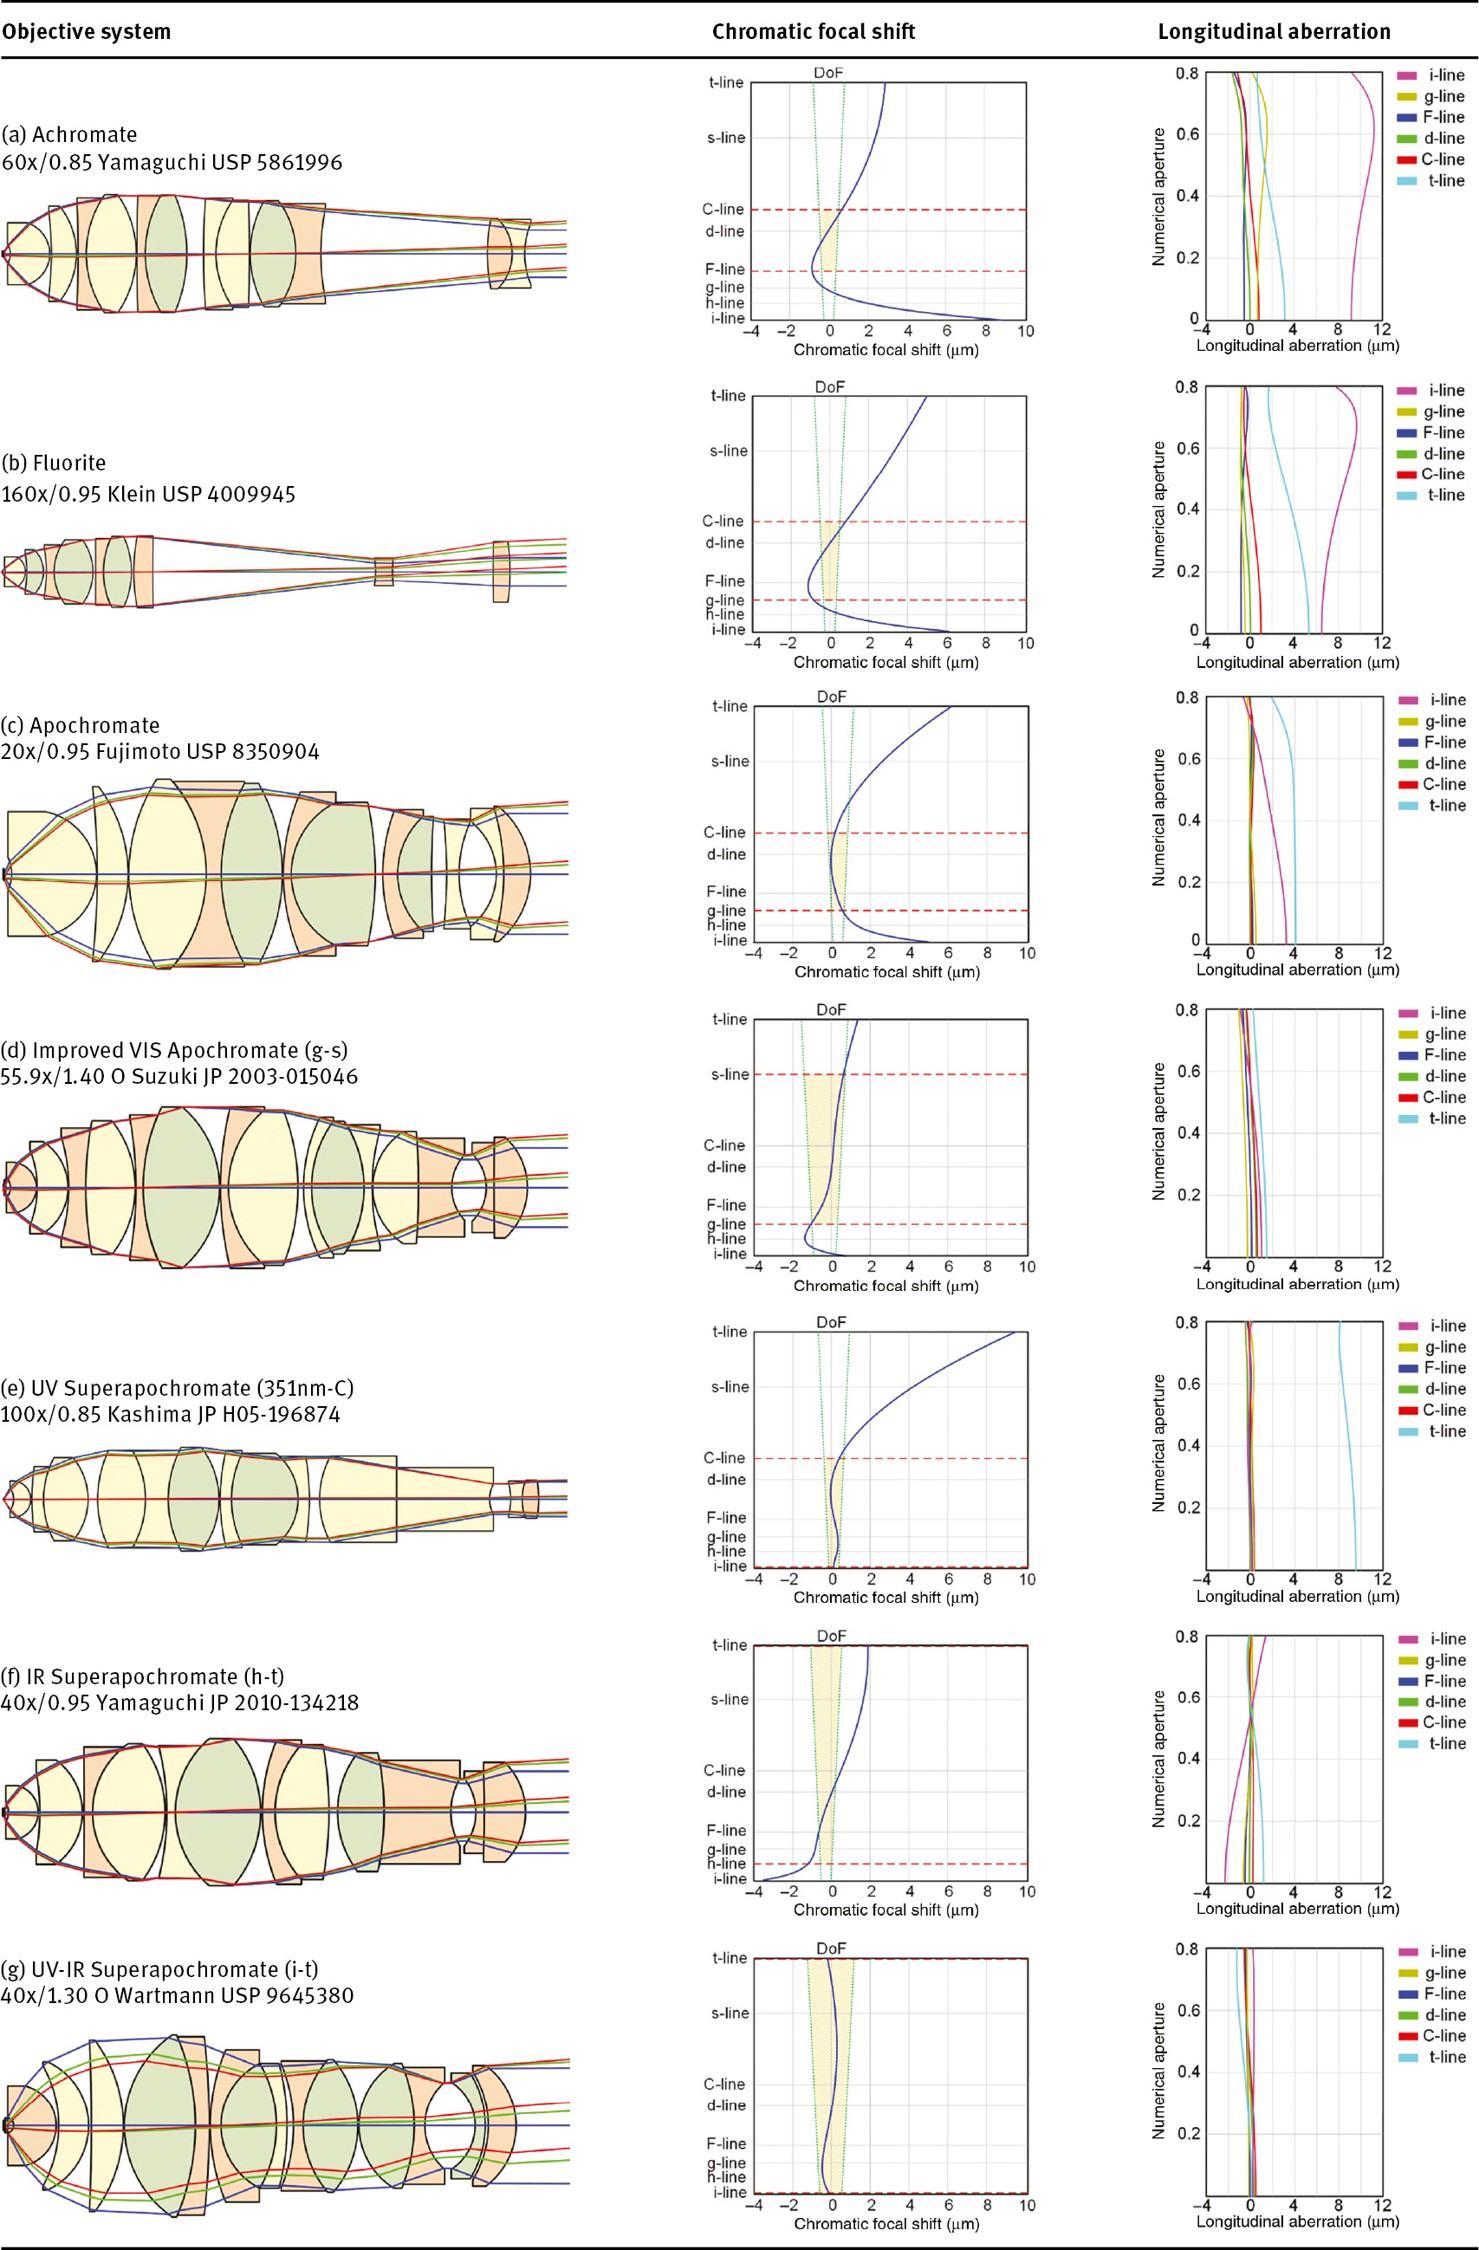
\includegraphics[width=\textwidth,height=0.72\textheight,keepaspectratio]{Figure/Zhang/ZhangFig_04.png}
                \label{fig:zhang_chromatic_classes}
            \end{figure}
        \end{column}
        \hfill
        \begin{column}{.42\textwidth}
            \textbf{这张图比较的不是“放大率”，而是\alert{色差校正等级}：}
            \begin{itemize}
                \item \textbf{Achromate}：通常校正两色，结构最简单
                \item \textbf{Fluorite / Semi-Apo}：三色校正更好，但仍有明显残余
                \item \textbf{Apochromate}：可把可见光范围内的纵向色差压到景深附近
                \item \textbf{VIS / UV / IR Superapo}：为扩展波段继续增加复杂度
            \end{itemize}

            \bigbreak
            \textbf{从右侧曲线看出的规律：}
            \begin{itemize}
                \item 校正等级越高，chromatic focal shift 曲线越平坦
                \item 不仅轴上色差更小，\alert{全孔径 spherochromatism} 也明显改善
                \item 扩展到 UV 或 IR 后，设计难度显著上升
            \end{itemize}

            \alert{结论：}“Apo”不是营销词，而是实打实对应\textbf{更多材料自由度、更复杂结构和更高制造成本}。
        \end{column}
    \end{columns}
\end{frame}
